\documentclass[preprint]{aastex}
\let\captionbox\relax
\usepackage{geometry}                % See geometry.pdf to learn the layout options. There are lots.
\geometry{letterpaper}                   % ... or a4paper or a5paper or ... 
%\geometry{landscape}                % Activate for for rotated page geometry
%\usepackage[parfill]{parskip}    % Activate to begin paragraphs with an empty line rather than an indent
\usepackage{graphicx}
\usepackage{hyperref}
\usepackage{amssymb}
\usepackage{epstopdf}
\usepackage[justification=centering]{caption}
\DeclareGraphicsRule{.tif}{png}{.png}{`convert #1 `dirname #1`/`basename #1 .tif`.png}

\makeatletter
\let\@dates\relax
\makeatother

\citestyle{aa}

\title{Planetary Astrophysics: \\ Homework 1}
\author{Samuel Factor}
%\date{\today}           % Activate to display a given date or no date

\begin{document}
\maketitle

\section{Question 1}
Code for my model can be found at \url{https://github.com/sfxfactor/PlanetaryHW1}. I implemented an \texttt{Orbit} object which stores the orbital parameters and the masses of the two bodies. There are then two methods associated with an \texttt{Orbit} object, \texttt{calcCoord} which, given a time or array of times, calculates the $X$, $Y$, and $Z$ coordinates along with $r$ and the 3 anomaly angles $f$, $E$ and $M$. The second method, \texttt{calcObs} calculates the observables given a time or array of times. This method returns the projected seperation and position angle of the two bodies, the projected seperation and position angle of each body with respect to the center of mass, the radial velocity of both objects as well as the coordinates returned by \texttt{calcCoord}.

\section{Question 2}

Orbital parameters of HD 80606 b from the literature are presented in Table \ref{tab:orbparams} along with sources. A plot of stellar radial velocity (RV) versus time spanning August 1 to December 31, 2015 (JD 2457235.5 to 2457387.5) is shown in Figure \ref{fig:RV}. The maximum and minum RV's occur on October 31 at 05:30 UT (JD 2457326.729) and November 1 at 22:35 UT (JD 2457328.441).

\begin{table}[h]
\begin{center}
    \caption{Orbital Parameters for HD 80606 b }\label{tab:orbparams} 
    \begin {tabular}{lcl}
    \tableline\tableline
    Parameter & Value & ref \\
    $a$ [AU] & $0.449\pm0.006$ & (1)\\
    $e$ & $0.9332\pm0.0008$ & (1)\\
    $i$ [$^\circ$] & $89.32\pm0.06$ & (1)\\
    $\Omega$ [deg] & (-19.02 or +160.98)$\pm0.45$ & (2)\\
    $\omega$ [deg] & $300.80\pm0.22$& (1)\\
    $t_0$ [JD] & $2454424.852\pm0.008$ & (1)\\
    $M_1$ [M$_\sun$] & $0.97\pm0.04$ & (1)\\
    $M_2$ [M$_\mathrm{jup}$] & $3.94\pm0.11$ & (1)\\
    \tableline
\end{tabular}
    \caption{Refrences: (1) \citet{orbparam}, (2) \citet{pol}}
\end{center}
\end{table}

\begin{figure}[h]
\begin{center}
    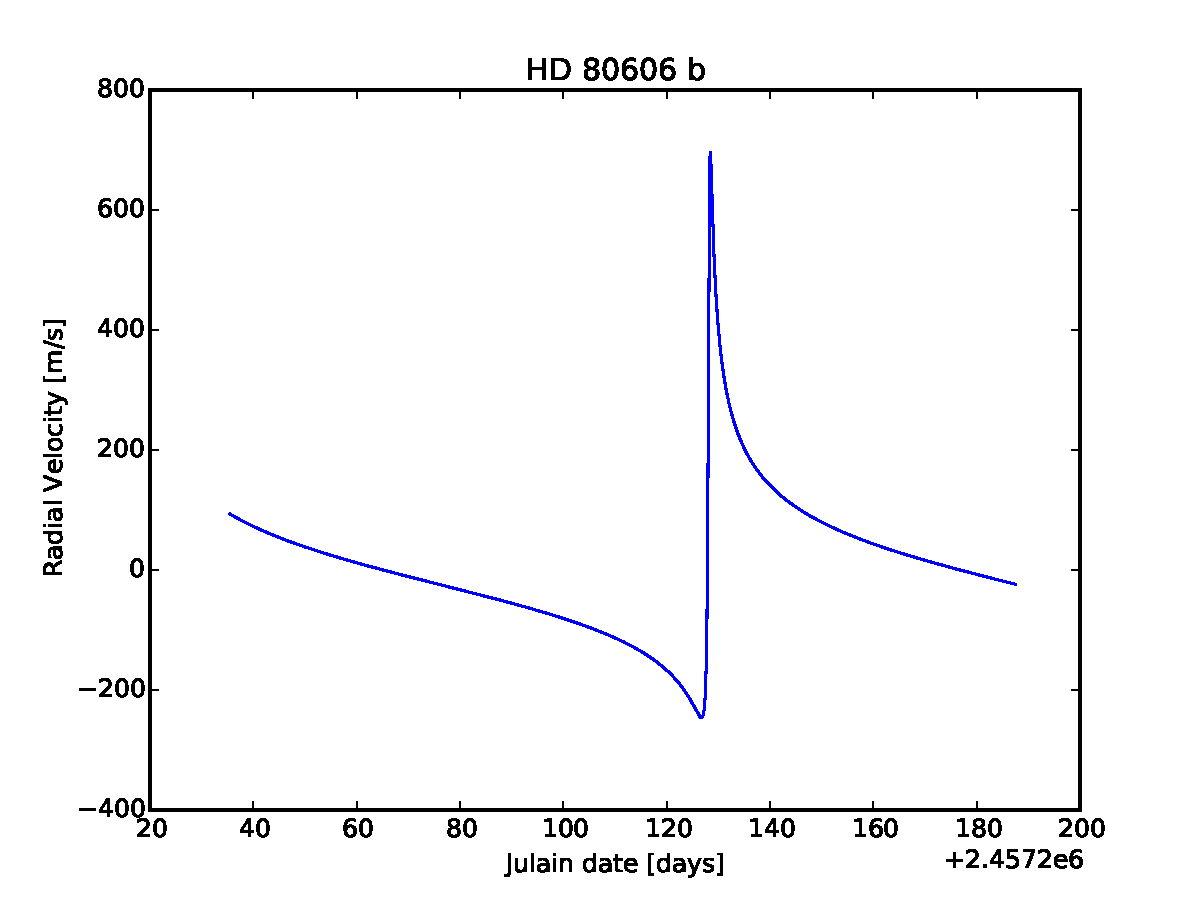
\includegraphics[width=\textwidth]{Q2.pdf}
    \caption{Radial velocity plot for HD 80606 b from August 1 to December 31, 2015}
    \label{fig:RV}
\end{center}
\end{figure}

\section{Question 3}

HD 80606 has a radius of $0.978\pm0.015 R_\sun$ \citep{orbparam}. The radius of the planet is $0.98\pm0.03 R_\mathrm{jup}$ \citep{orbparam}. With this information we can calculate when the projected seperation of the planet and star would result in a transit. First and fourth contact occur when the projected seperation is equal to the sum of the radii. The first transit occurs on November 1 12:03-13:56 UT (JD 2457328.002-2457328.081) and the second occurs on November 7 02:51-15:20 UT (JD 2457333.691-2457334.139). The first transit occurs from 6-8 am which would not be observable. The second occurs from 9pm to 9am which would be visible from McDonald. Though the fact that the altitude of HD 80606 does not get above $30^\circ$ unitl about 2 am and the sun rises much before 9 am means that the data will be limited. Second contact occurs at 23:24 and third occurs just before 07:00 which means we will not be able to observe ingress/egress.

\section{Question 4}

The end-of-mission sky-average astrometric performance for a bright G2V star is 6.7 $\mu$as \citep{gaia}. 
HD 80606 was observed by the Hipparcos satalite to have a paralax of $17\pm6$ mas, corresponding to a distance of $60\pm20$ pc. 
The parallactic motion was calculated using equations from \citet{parallax}.

\begin{figure}
\begin{center}
    \includegraphics[width=\textwidth]{1radec.pdf}
    \caption{DEC versus RA offset from the center of mass of the system accounting only for reflex motion for 100 observations sampled randomly from the 5 year Gaia science mission. Error bars are the expected 6.7 $\mu$as precision. }
    \label{fig:1radec}
\end{center}
\end{figure}

\begin{figure}
\begin{center}
    \includegraphics[width=\textwidth]{1time.pdf}
    \caption{RA and DEC versus time for the same points as in Fig. \ref{fig:1radec}.}
    \label{fig:1time}
\end{center}
\end{figure}

\begin{figure}
\begin{center}
    \includegraphics[width=\textwidth]{2radec.pdf}
    \caption{Same as Fig. \ref{fig:1radec} but also accounting for motion due toparallax.}
    \label{fig:2radec}
\end{center}
\end{figure}

\begin{figure}
\begin{center}
    \includegraphics[width=\textwidth]{2time.pdf}
    \caption{Same as Fig \ref{fig:1time} but also accounting for motion due to parallax.}
    \label{fig:2time}
\end{center}
\end{figure}

\begin{figure}
\begin{center}
    \includegraphics[width=\textwidth]{3radec.pdf}
    \caption{Same as Fig \ref{fig:2radec} but also accounting for propper motion.}
    \label{fig:3radec}
\end{center}
\end{figure}

\begin{figure}
\begin{center}
    \includegraphics[width=\textwidth]{3time.pdf}
    \caption{Same as Fig \ref{fig:2time} but also accounting for propper motion.}
    \label{fig:3time}
\end{center}
\end{figure}


\bibliographystyle{apj}
\bibliography{sources}

%\subsection{}

\end{document}  
